\documentclass{standalone}

\usepackage{tikz}
\usepackage{tikz-3dplot}
\usetikzlibrary{decorations.pathreplacing}%使用大括号
\usetikzlibrary{calligraphy} %calligraphy 书法风格
% \usetikzlibrary{positioning}
\usetikzlibrary{calc}
\usetikzlibrary{backgrounds} %特定的绘图操作置于背景层
\usetikzlibrary{3d}
\begin{document}
%圆锥展开图
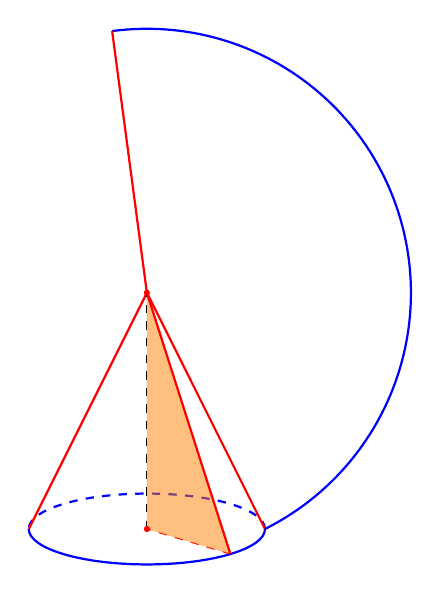
\begin{tikzpicture}[scale=1.5,
    y={(0cm,-0.3cm)}, % 设置 x 轴方向
    x={(1cm,0cm)},            % 设置 y 轴方向
    z={(0cm,1cm)}             % 设置 z 轴方向
]
    % 定义圆柱的参数
    \def\radius{1} % 圆锥底面半径
    \def\height{2} % 圆锥的高度
    \pgfmathsetmacro{\expandradius}{sqrt(\radius*\radius + \height *\height)} %展开图弧长

    \pgfmathsetmacro{\expandarc}{2*pi*\radius/\expandradius} %展开图圆心角

    \pgfmathsetmacro{\resultAtan}{atan(\radius / \height )}
    % 将弧度转换为角度

    % 一些坐标
    \coordinate (O') at (0,0,\height);
    \coordinate (O) at (0,0,0);
    %上圆上一点
    \coordinate (A') at ({\radius*sqrt(2)/2},{\radius*sqrt(2)/2},\height);
    %下圆上一点
    \coordinate (A) at ({\radius*sqrt(2)/2},{\radius*sqrt(2)/2},0);
        % 底面半径
        \draw[thin,dashed,red] (A) -- (O);
        % 绘制底面圆
        \begin{scope}
            \draw [blue,thick,dashed] (\radius,0,0) arc (0:-180:\radius) ;
            \draw [blue,thick] (\radius,0,0) arc (0:180:\radius) ;

        \end{scope}
        \fill[orange,opacity=0.5] (A) -- (O) -- (O') -- cycle;
        % 绘制母线
        \begin{scope}
            \draw[thick,red] (\radius,0,0) -- (O');
            \draw[thick,red] (-\radius,0,0) -- (O');
            \draw[thick,red] (A) -- (O');
        \end{scope}
        

        % 绘制高线
        \begin{scope}
            \draw[thin,dashed] (0,0,0) -- (0,0,\height);
            \fill[red] (0,0,0) circle (0.75pt);  % 绘制一个点测试一下 
            \fill[red] (0,0,\height) circle (0.75pt);  % 绘制一个点测试一下 
        \end{scope}


    % 绘制展开图圆弧
    \begin{scope}[canvas is xz plane at y=0]
        % \draw [blue,thick] (\radius,0,0) arc [start angle=-\expandarc/2 r, end angle=\expandarc/2 r, radius=\expandradius];
        \draw[blue, thick] plot[domain=0 r:\expandarc r,samples=100] ({\expandradius*cos(\x - pi/2 r +\resultAtan )},{\expandradius*sin(\x - pi/2 r +\resultAtan  )+\height});
    \end{scope}

    % - pi r +\atan(\radius/\height) r

    % 绘制展开图扇形的边
    \begin{scope}
        % \draw[thick,red] (\radius,0,2 *\height) -- (O');
        \draw[thick,red] ({\expandradius*cos(\expandarc r - pi/2 r +\resultAtan )},0,{\expandradius*sin(\expandarc r - pi/2 r +\resultAtan  )+\height}) -- (O');
        % \draw[thick,red] (-\radius,0,0) -- (O');
        % \draw[thick,red] (A) -- (O');
    \end{scope}

    % \node[red, align=center] at (4,0) {\expandradius};
    % \node[red, align=center] at (4,1) { \pgfmathatan{1} \pgfmathresult};
\end{tikzpicture}
\end{document}    